\section{Alternative Cost Functions}\label{app:alternative_costs}

We next show that regions of differing responses between behavioral and non-behavioral agents, similar to those depicted in Figure~\ref{fig:highlighted}, will also emerge under quadratic and weighted Manhattan cost functions. We also describe the cost function presented to users' in our experiments, which can be viewed as an approximation of a quadratic cost.

\paragraph{Quadratic Cost Function.}
The following lemma characterizes the post-strategic features under the quadratic cost $c(\vx, \vx_0)=\sum_i c_i(x_{i}-x_{i,0})^2$.
\begin{lemma}\label{lemma:quad-cost-band}
    Let $\mC$ denote a diagonal matrix with $c_i$'s as its diagonal, and let $\vy$ denote the feature vectors satisfying $\vtheta^T\vy = \theta_0$. For an agent with starting feature vector $\vx_0$, if $\vx_0$ is in the n-dimensional ellipsoid determined by $B$ and $\mC$, i.e., if $(\vy-\vx_0)^T\mC (\vy-\vx_0)\le B$,
    \begin{align*}
        x_{\text{NB}, i} = \frac{\theta_{0}-\vtheta^T\vx_0}{\sum_j \frac{\theta_j^2}{c_j}}\cdot \frac{\theta_i}{c_i}+x_{0,i}~.
    \end{align*}
    Otherwise, $\vx_\text{NB}=\vx_0$. For behaviorally biased agents, $\vx_\text{B}$ is obtained similarly by replacing $\vtheta$ with $\vw(\vtheta)$.
\end{lemma}

Figure~\ref{fig:BR-illustration-quad-cost} illustrates the best-responses of Lemma~\ref{lemma:quad-cost-band} for rational (non-behavioral) and biased (behavioral) agents. Specifically, the condition in Lemma~\ref{lemma:quad-cost-band} constructs an $n$-dimensional ellipsoid around every point on the line $\vtheta^T\vx = \theta_{0}$, containing agents who have sufficient budget to strategically change their features to reach that particular point on the boundary, with the coefficients $c_i$ determining the scaling along each axis. %For $c_i=c, \forall i$, the ellipsoid becomes an n-dimensional sphere; for $c=1$, the cost becomes the norm-2 cost. 
Since the scaling of the ellipsoid does not depend on the point of the line we are focusing on, the union of these ellipsoids (determining the set of all agents who can afford to be classified positively through gaming) forms a band below the line $\vtheta^T\vx=\theta_0$. Note that this band differs from the one in Lemma~\ref{lemma:band-optimization}. 

\begin{figure}[ht]
    \centering
    \begin{subfigure}[t]{0.22\textwidth}
        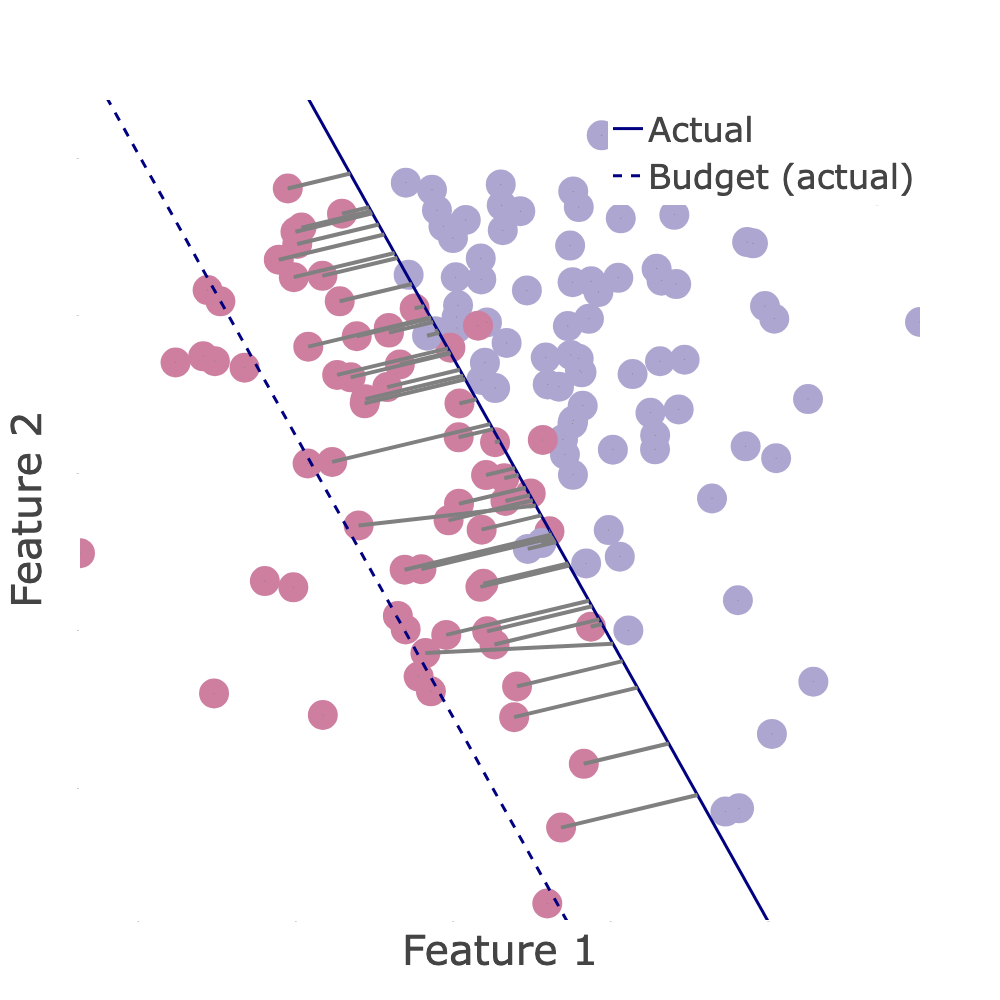
\includegraphics[width=0.9\textwidth]{Figures/quad-NB.png}
            \caption{Rational response}
            \Description[Rational response under quadratic cost]{This figure shows the rational response of agents to a known threshold classifier in 2 dimensions under quadratic cost.}
        \label{fig:NB-arrows-quad-cost}
    \end{subfigure}
    \hspace{0.01in}
    \begin{subfigure}[t]{0.22\textwidth}
        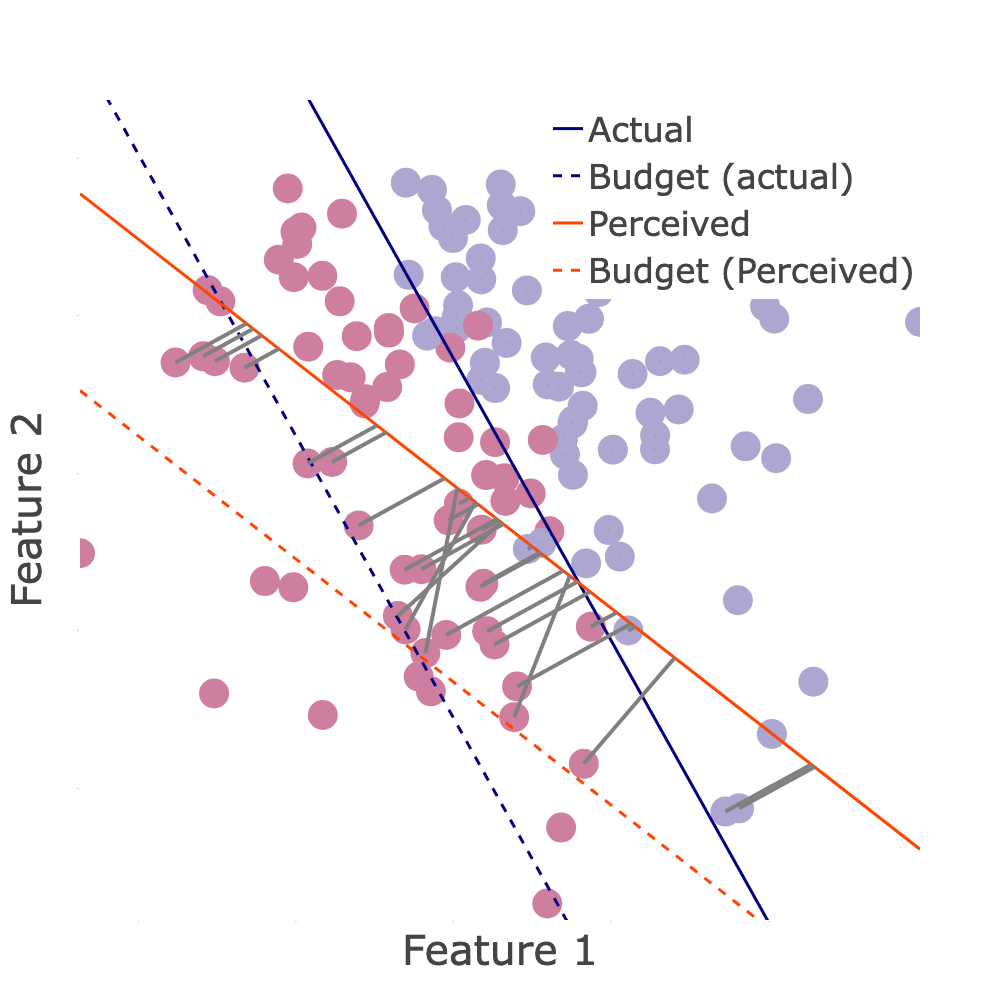
\includegraphics[width=0.9\textwidth]{Figures/quad-B.png}
        \caption{Biased response}
        \Description[Biased response under quadratic cost]{This figure shows the biased response of agents to a known threshold classifier in 2 dimensions under quadratic cost.}
        \label{fig:B-arrows-quad-cost}
    \end{subfigure}
    \caption{Strategic responses under quadratic costs.}
    \Description[Responses under quadratic cost]{This figure shows the responses of agents to a known threshold classifier in 2 dimensions under quadratic cost.}
    \label{fig:BR-illustration-quad-cost}
\end{figure} 

\paragraph{Weighted Manhattan Distance Cost Function.}
The following lemma characterizes the post-strategic features under the weighted Manhattan cost $c(\vx, \vx_0)=\sum_i c_i|x_{i}-x_{i,0}|$.
\begin{lemma}\label{lemma:manhattan-cost-band}
    Let $\ve_i$ be the unit vector with 1 in the $i$\textsuperscript{th} coordinate and 0 elsewhere, and $k = \arg\min_i \frac{c_i}{\theta_i}$. For an agent with starting feature $\vx_0$, if $\vtheta^T\vx_0 + \frac{\theta_k}{c_k}B \ge \theta_0$,
    \begin{align*}
        \vx_\text{NB} = \vx_0 + (\theta_0-\vtheta^T\vx_0)\frac{c_k}{\theta_k}\ve_k~.
    \end{align*}
    Otherwise, $\vx_\text{NB}=\vx_0$. For behaviorally biased agents, $\vx_\text{B}$ is obtained similarly by replacing $\vtheta$ with $\vw(\vtheta)$.
\end{lemma}

Figure~\ref{fig:BR-illustration-lin-cost} illustrates the best-responses of Lemma~\ref{lemma:manhattan-cost-band} for rational (non-behavioral) and biased (behavioral) agents.
Again, the set of agents who can afford to game the system to receive a positive classification, as identified in Lemma~\ref{lemma:manhattan-cost-band}, is a band below the classifier (but different from those of Lemmas~\ref{lemma:band-optimization} and \ref{lemma:quad-cost-band}). In particular, under this cost, agents spend all their budget on changing the feature with the most ``bang-for-the-buck'' $\frac{c_i}{\theta_i}$ (or perceived bang-for-the-buck $\frac{c_i}{w_i(\vtheta)}$). As seen in the two-dimensional illustration in Figure~\ref{fig:BR-illustration-lin-cost}, this means that while it is optimal for rational agents to invest only in feature 2, those with behavioral bias believe feature 1 has a better return, leading to a sub-optimal response by them. We also note that even though the movements of agents in the specified band are different from the movement for the norm-2 cost, the bands form the same regions of differing responses as in Figure~\ref{fig:BR-illustration}, where agents overshoot, undershoot, do nothing at all, or needlessly change their features, when they are behaviorally biased. 

\begin{figure}[ht]
    \centering
    \begin{subfigure}[t]{0.22\textwidth}
        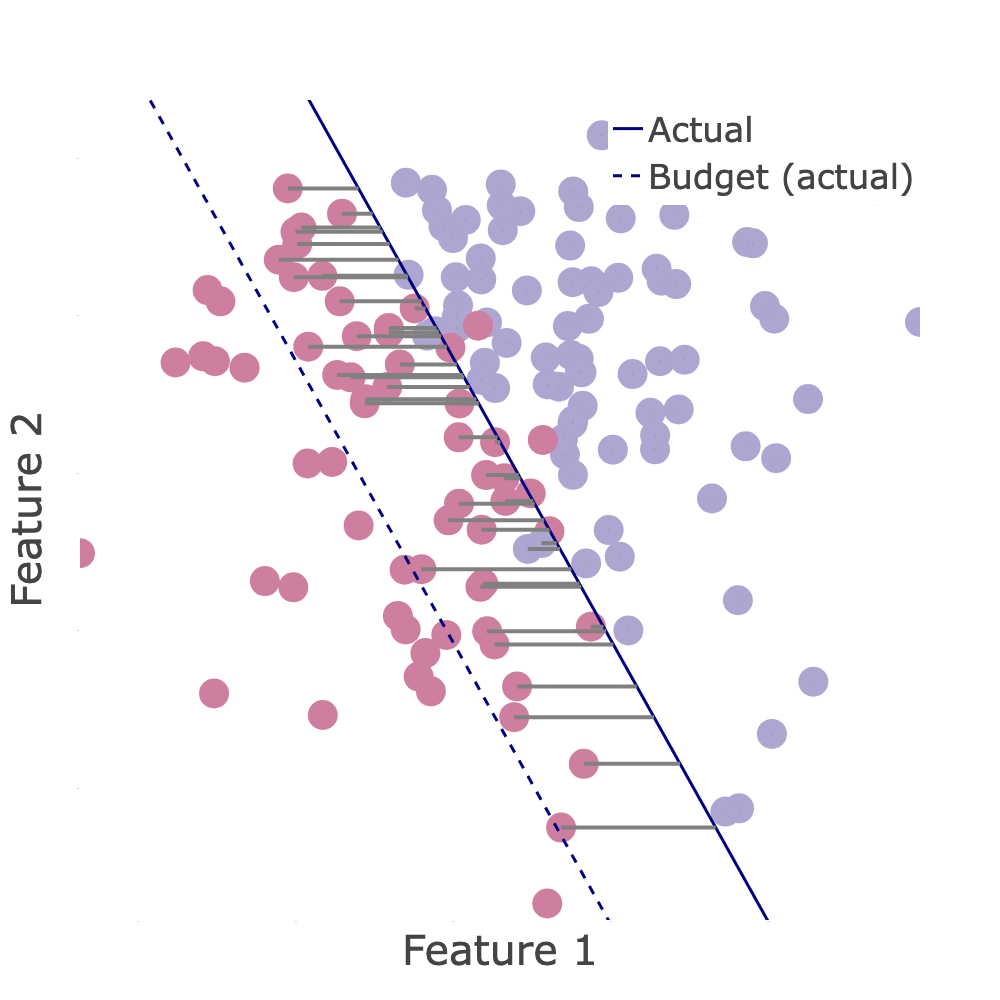
\includegraphics[width=0.9\textwidth]{Figures/lin-NB.png}
            \caption{Rational response}
            \Description[Rational response under Manhattan cost]{This figure shows the rational response of agents to a known threshold classifier in 2 dimensions under Manhattan cost.}
        \label{fig:NB-arrows-lin-cost}
    \end{subfigure}
    \hspace{0.01in}
    \begin{subfigure}[t]{0.22\textwidth}
        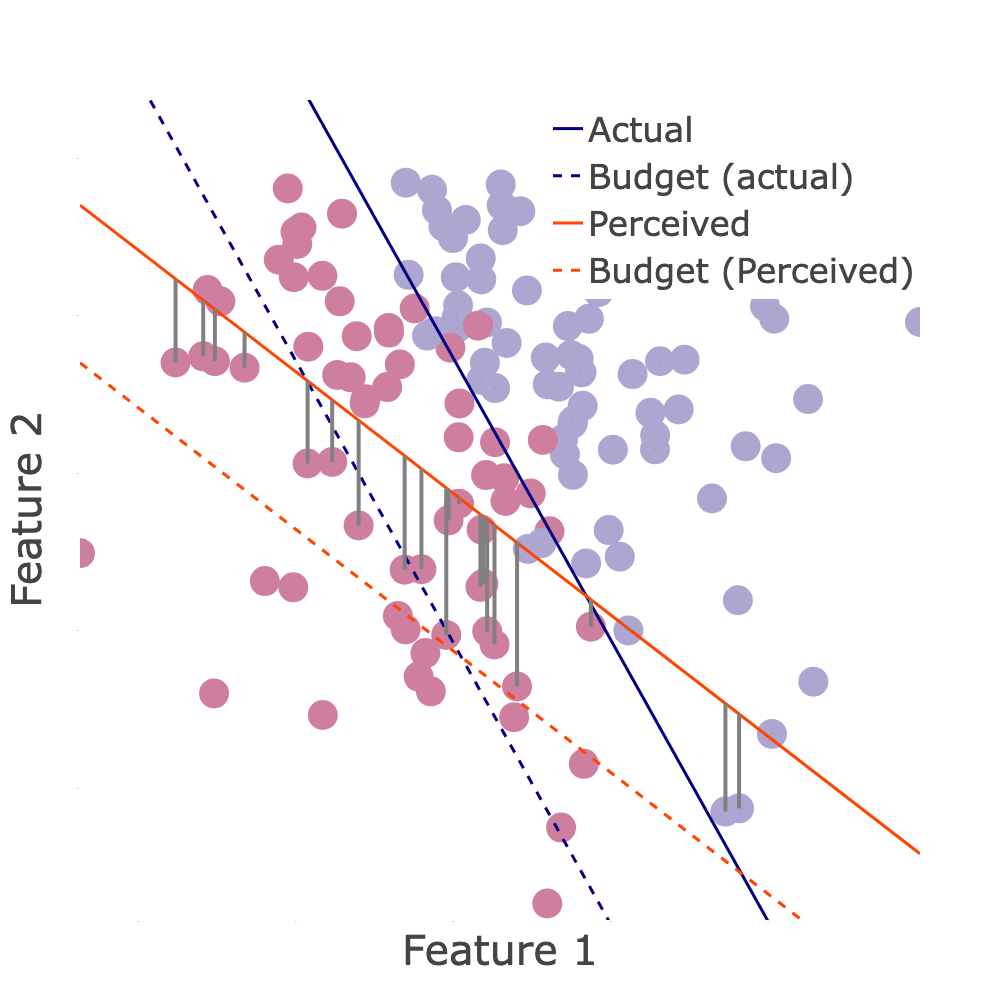
\includegraphics[width=0.9\textwidth]{Figures/lin-B.png}
        \caption{Biased response}
        \Description[Biased response under Manhattan cost]{This figure shows the biased response of agents to a known threshold classifier in 2 dimensions under Manhattan cost.}
        \label{fig:B-arrows-lin-cost}
    \end{subfigure}
    \caption{Strategic responses under Manhattan costs.}
    \Description[Responses under quadratic cost]{This figure shows the responses of agents to a known threshold classifier in 2 dimensions under Manhattan cost.}
    \label{fig:BR-illustration-lin-cost}
\end{figure}  

\paragraph{Cost Function in the User Studies.} For our human subject experiments in Section~\ref{sec:user-study}, to provide simple, yet actionable information to  participants, without the need for them to understand a specific form of cost function, we describe the cost of changing features to participants through a \emph{piecewise linear cost function}. This can be viewed as an approximation of a quadratic cost using a step function with a weighted Manhattan cost at each step, with the approximation improving as the number of steps increases (see the two-dimensional illustration in Figure~\ref{fig:2d-approx-illustration}). Specifically, in our user experiments, we break the budget $B$ into three steps of increments $B_1$, $B_2$, and $B_3$ with $B_1+B_2+B_3=B$, and assign a constant cost $c_1$, $c_2$, and $c_3$ for changing features at each increment. This means that in each step, agents face a weighted Manhattan cost, but overall, the cost is not fixed, and investing in a single feature is not optimal. 

\begin{figure}[ht]
    \centering
    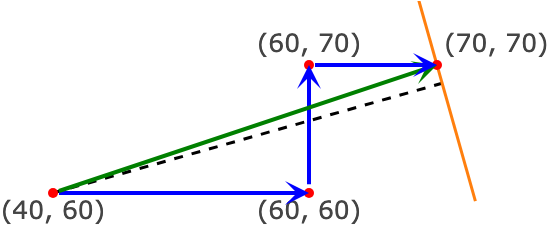
\includegraphics[width=0.8\linewidth]{Figures/illustration-single-movement.png}
    \caption{Strategic responses under a quadratic cost (green) vs. a piece-wise linear cost function (blue).}
    \Description[Responses under various costs]{This figure shows the responses of agents to a known threshold classifier in 2 dimensions under various costs with a numerical example.}
    \label{fig:2d-approx-illustration}
\end{figure}

\paragraph{More general cost functions.} We note that using more complex and general cost functions is possible. Specifically, the cost function impacts the movement trajectory of each point (agent), and while different cost functions might result in variations in the specific trajectories, the overall structure of the generic regions can remain unchanged; this is what we have observed with the $l_1$ and $l_2$ step costs functions. %For other $l_p$ norms with $p>1$ we see a different trajectory for each agent's movement but will again give us the same regions as in Figure~\ref{fig:highlighted}; the detailed analysis on cost functions is provided in Appendix~\ref{app:alternative_costs}.}

{Similarly, for $l_p$ norm cost functions we can see that the trajectory of an agent starting from $\vx_0$ is given by:
\begin{align}
    x_i = x_{0,i} - \frac{\vtheta^T\vx_0 - \theta_0}{\sum_i \frac{\theta_i^2}{|x_i-x_{0,i}^{p-2}|}}\times \frac{\theta_i}{|x_i-x_{0,i}^{p-2}|}~,
\end{align}
which will give us similar regions as shown in Figure~\ref{fig:highlighted}. That said, it is also not hard to find specific cost functions that might change the agents' trajectories in a way that alters the regions in Figure~\ref{fig:highlighted}. For instance, a fixed cost function $c(\vx,\vx_0) = c$, for all $\vx\neq\vx_0$, will allow the agents that can afford to manipulate their features to move to the decision boundary in whichever way they want. This can lead to expanding region 4 in Figure~\ref{fig:highlighted} to include regions 2 and 3. We view the analysis under such cost functions (those for which the 6 distinct regions in Figure~\ref{fig:highlighted} do not emerge) as a promising direction for future research.}